\documentclass[a4paper,11pt]{article}
\usepackage[latin1]{inputenc}
\usepackage[T1]{fontenc}
\usepackage[english]{babel}
% \usepackage{amsmath}
% \usepackage{amssymb,amsfonts,textcomp}
% \usepackage{color}
% \usepackage{array}
% \usepackage{supertabular}
% \usepackage{hhline}
\usepackage{hyperref}
\usepackage{cite}
% \usepackage{etoolbox}
\usepackage{acro}
\usepackage{graphicx}
\usepackage[nodayofweek]{datetime}

\acsetup{first-style=short}
\DeclareAcronym{hls}{
  short = HLS ,
  long  = Hue Lightness Saturation,
  class = abbrev
}
\DeclareAcronym{hgr}{
  short = HGR ,
  long  = Hand Gesture Recognition,
  class = abbrev
  }

  \DeclareAcronym{opencv}{
  short = OpenCV ,
  long  = Open Computer Vision,
  class = abbrev
  }

  \DeclareAcronym{hci}{
  short = HCI ,
  long  = Human Computer Interaction,
  class = abbrev
  }


\DeclareGraphicsRule{*}{mps}{*}{}
\newcommand{\mparagraph}[1]{\paragraph{#1}\mbox{}\\}

% Commands
\newcommand{\HRule}{\rule{\linewidth}{0.5mm}} % Defines a new command for the horizontal lines

\begin{document}

	\begin{titlepage}
		\begin{centering}
		 
		%	HEADING SECTIONS
		\textbf{\textit{\large{B.Tech Project Report}}}\\[0.5cm]
		
		\textsc{\textbf{\LARGE{Gesture recognition for controlling vlc media player}}}\\[1.5cm]

		\large{Submitted in partial fulfilment for the award of the Degree of Bachelor of Technology in Computer Science and Engineering}\\[1.5cm]

		\large{Submitted by}\\[0.5cm]

		\textbf{Chithra     (Roll No 13400020)}\\
		\textbf{Sindoora N     (Roll No 13400056)}\\
		\textbf{Krishna Prabha R    (Roll No 13400071)}\\[1.5cm]
		
		{Under the guidance of}\\[0.25cm]
		\large{Ms. Rajasree R.}\\[0.5cm]

		
\includegraphics[width=5cm]{images/logo.jpg} 

		Department of Computer Science and Engineering\\
		\textsc{College of Engineering, Trivandrum}\\
		\textsc{Kerala}\\
		\textsc{May 2017}\\
		\vfill % Fill the rest of the page with whitespace
		\end{centering}
	\end{titlepage}

	\begin{titlepage}
		\begin{centering}
			\textbf{\textit{\LARGE\textsc{{certificate}}}}\\[0.5cm]
			
\includegraphics[width=5cm]{images/logo.jpg}\\

		\end{centering}

		\large{This is to certify that the thesis entitled ``Gesture recognition for controlling VLC media player'' is a bonafide record of the major project done by \textbf{Chithra} (Roll No 13400020), \textbf{Sindoora N} (Roll No 13400056) and \textbf{Krishna Prabha R} (Roll No 13400071) under my supervision and guidance, in partial fulfilment for the award of the Degree of Bachelor of Technology in Computer Science and Engineering from the University of Kerala for the year 2017.}\\[1.5cm]

		\begin{minipage}{0.4\textwidth}
		\begin{flushleft}
		\end{flushleft}
		\end{minipage}
		~
		\begin{minipage}{0.6\textwidth}
		\begin{centering} \large
		\large{Ms. Rajasree R}\\
		\small{(Guide)}\\
		\small{\textit{\textbf{Asst. Professor}}}\\
		\small{\textit{\textbf{Dept. of Computer Science and Engineering}}}\\[1.5cm]

		\large{Mrs. Liji}\\
		\small{\textit{\textbf{Professor and Head}}}\\
		\small{\textit{\textbf{Dept. of Computer Science and Engineering}}}\\
		\end{centering}
		\end{minipage}\\[1.0cm]

		\begin{flushleft}
		Place: Trivandrum\\
		Date:  11-05-2017\\
		\end{flushleft}
		\vfill % Fill the rest of the page with whitespace
	\end{titlepage}

	% TODO Ack before this
	\pagenumbering{roman}
	
	\begin{abstract}
		The computer is more important in our daily life. Computer applications require interactions between human and computer.This interaction needs to be unrestricted and it has made challengeable  to traditional input devices such as keyboard, mouse, pen etc. Some factors  of  communication like facial expressions, eye contact,  are  already  being  used  to  interact  with  computer  and  other systems. Some  examples  are  face  detection,  speech  recognition  system,  retina  scanning  biometrics  and motion detection  sensors.  But  one  of  the  most
		common  elements  of  communication  is  not  widely  used  for  computer  interaction,  hand  gesture.  We  often  use  hand  gesture  in  communication  with  people  in  real  world,  we can  use  hand 
		gesture  to  interact  with  the  digital  world  also.  This  will  give  the  field  of  Human  Computer  Interaction  the  natural method to interact with computer systems, and will make interaction with computer more real-life and easy.

		 Hand gesture is an  important  component  of  body  languages  in  linguistics.  Human  computer  interaction  becomes  easy  with  use  of  hand  as  a  device. Hand  gestures  are  used  to control various applications like VLC media player, robot control, gaming etc. 

		

		In this project, we are using the gestures to control the media player. For that, we use the webcamera to detect gestures made by the user. The camera captures this and identifies the gesture, recognises it against a set of known gestures and performs the basic operations of VLC media player corresponding to it. 

		To make this project a reality, we have used C++ language, openCV library for image processing and the VLC library for VLC functions. When we show our hand against the camera, the average colour of the hand is detected, and the background is eliminated accordingly using the skin colour detection algorithm. Then the contours of the hand is found with the help of convex hull and convexity defect techniques. Also the fingertips are tracked. By recognising the movement of the centroid and coordinates of the fingertips of the gesture, stored gesture type is identified and returned. The action corresponding to the returned value is executed.


	\end{abstract}
	
	\newpage
	\tableofcontents
	\newpage
	\listoffigures
	\newpage
	\printacronyms[include-classes=abbrev,name=Abbreviations]
	\newpage

	\pagenumbering{arabic}
	\section{Introduction}
		
		Gesture recognition is gaining so much importance nowadays. In this system, as we have used gestures as a medium for communicating with the computer, we need to know about the gestures. Gestures can be defined by body, or hand movements. Gestures can be of static or dynamic type. In this, we have used dynamic hand gestures for the control of application.

		Gestures can originate from any bodily motion or state but commonly originate from the face or hand. Current focuses in the field include emotion recognition from face and hand gesture recognition. Users can use simple gestures to control or interact with devices without physically touching them. Many approaches have been made using cameras and computer vision algorithms to interpret sign language. However, the identification and recognition of posture, gait, proxemics, and human behaviors is also the subject of gesture recognition techniques.[1] Gesture recognition can be seen as a way for computers to begin to understand human body language, thus building a richer bridge between machines and humans than primitive text user interfaces or even GUIs (graphical user interfaces), which still limit the majority of input to keyboard and mouse.
		\subsection{Motivation and Overview}
		
			Gesture, being a most important factor in linguistic communication, we thought of enhancing those to the computer world too. The main motivation behind this project is to make the machine interface more flexible and more easy for the user. There are many applications where gesture recognition can find application, we have used the VLC media player, the most commonly used player for watching videos, movies etc.

			The project deals with the detection of the hand gesture and tracking of movement of the gesture. Video fed from webcamera is used for recognition. Recognition mainly constitutes of hand detection and feature extraction. Our gesture recognition system assume static background. In our system, we created a gesture recognition that works on varying illumination condition. To extract the hand from the frame, we used robust skin detection algorithm.

			 As there is no static gesture used in the commands, the motion of the centroid and fingertips with respect to the frames are tracked. Then the gesture mapped to the functions associated with the vlc media player is compared and executed accordingly.


		\subsection{Background and Literature Survey}
			Gesture recognition system was introduced into the digital world inspired by the sign language used by the disabled people. Researchers realised that these signs can be used to offer simple command to a computer interface. This gradually evolved with a much developed accelerometer, infrared cameras and even fibre-optic bend sensors.




			% \paragraph{Deep Mind and Reinforcement Learning} 
	\section{Materials and Methodology}
		\subsection{Algorithms}
			\subsubsection{Skin detection algorithm}	
				Detection of skin in video is an important component of systems for detecting, recognizing, and tracking faces and hands. Different skin detection methods have used different color spaces. We are using HLS colour space. Thus every colour image is composed of three planes namely Hue, Lightness and Saturation (HLS). To extract the hand from the image foreground image is decomposed into H, L and S planes.
				
				When the camera opens, we have to show our hand in the requested region.  Once the image is captured and when the image is separated in to frames, skin detection algorithm is applied to allocate the skin from the background images. That is, a number of frames are taken and in each of the frame the median of each H L and S components are identified. Then if a particular colour comes in any one of the frame as a median, it is extracted as a part of the image. We took the median as a method of detecting the skin colour because that colour obtained as the median will be the major colour got in that frame in the region where the hand is shown. 

				Thus the average colour is taken for proceeding to the further steps.


		\subsection{Program Development}
			When the webcamera captures the gestures, it is converted into many frames and the median colour of the skin is determined using the previously mentioned skin detection algorithm. The average colour found out is stored as a scalar value containing separate components of hue, lightness and saturation. After that each of the following steps are executed.
		\subsubsection{Filtering}
			Once the skin colour have been detected, the next step is to determine which region corresponds to hand and which region corresponds to noise. Then the found out average colour is added with a particular predefined HLS values and is made as the upper bound. Also, the same predefined HLS values are subtracted from the average colour to find the lower bound. Any colour that comes between this range is detected as a high boolean value, and all others are treated to be zero. The region that comes within this range of colours are made as white and the rest of the image made black.  A nonlinear median filter is then applied to get a smooth and noise free binary representation of the hand. In our project binary image is also displayed to know whether the threshold has been taken correctly.

			\subsubsection{Contours and fingertip detection}
				% \paragraph{Neural Networks}
				After skin detection, there are possibilities that there are small noisy regions. So we first extract the contours of all the detected skin regions using the binary image obtained from filtering process mentioned above. We assume that the largest skin region is our hand. So from all the obtained contours, we first find the region with the largest contour, which is the required region. And the index of the contour is also stored. 

				Initially, we compute the convex hulls for the set of points corresponding to contours of hand. The convex hull is used to find the envelope of set of points of contours we detected earlier in the region extraction step. In each of these convex hull, we compute the convexity defects. We then eliminate the unwanted defects by setting a tolerance value of angle and depth. Also the points within the close proximity are also eliminated.

				Now after the convexity defects are also found out, number of fingers and coordinates of the fingertips are tracked. This is found with the help of the returned values from the convex hull method. Then the fingertips are stored for the future values.
			\subsubsection{Gesture recognition and command execution}
				Gestures are recognised with the help of the centroid and movement of the fingertips. For that, the centroid of the given region is to be found out within each frame. That is, the centroid with reference to the previous frames are identified to find the movement. Also some gestures without changing the centroid are also defined. For those gestures, movement of the fingertip coordinates are checked. 

				Whenever a gesture is recognised, if there is a command which is defined for a VLC operation is obtained which matches to the recognised gesture, that command value is returned and executed.

				The defined commands are as follows:
				Centroid moving to the right: Play the video.
				Centroid moving to the left: Pause
				Fingertips moving to the right with no large deviation in centroid: Forward
				Fingertips moving to the left with no large deviation in centroid: Stop

			 \subsection{System Description}

			 	The primary goal of the gesture recognition is to create a system which can identify
specific human gestures and use them to convey information for controlling various applications. The method considered suitable for gesture recognition is to use
vision sensors like cameras to acquire images, which are analysed to recognise the gestures.
Also non-gesture recognition system increases the cost and unnecessary hardware while
this sensorless system is less costly and also efficient to use. This could make conventional
input devices such as mouse, keyboards and even touch-screens redundant.
			 	Gesture recognition is done with the help of image processing and computer vision. Image processing is processing of images using mathematical operations by using any form of signal processing for which the input is an image, a series of images, or a video, such as a photograph or video frame. The output of image processing may be either an image or a set of characteristics or parameters related to the image.

			 	 Computer vision is an interdisciplinary field that deals with how computers can be made for gaining high-level understanding from digital images or videos. From the perspective of engineering, it seeks to automate tasks that the human visual system can do. Computer vision tasks include methods for acquiring, processing, analyzing and understanding digital images, and extraction of high-dimensional data from the real world in order to produce numerical or symbolic information.

			 	 We have used OpenCV library to deal with the image processing tasks. OpenCV (Open Source Computer Vision) is a library of programming functions mainly aimed at real-time computer vision.
			 	 . It can detect and recognize a large variety of objects, but our focus now is to apply techniques and methods to detect and recognize the gestures of a human hand. C++ is the programming language that we have used to implement this system as we were more comfortable with this language. We had to implement certain features of our own as in built libraries and associated functions were not available with this language. Although there were limitations, we were successful in building a simple form of gesture recognition system. \\
			\subsubsection{Class Diagram}
			\begin{figure}[!ht]
			\begin{centering}
				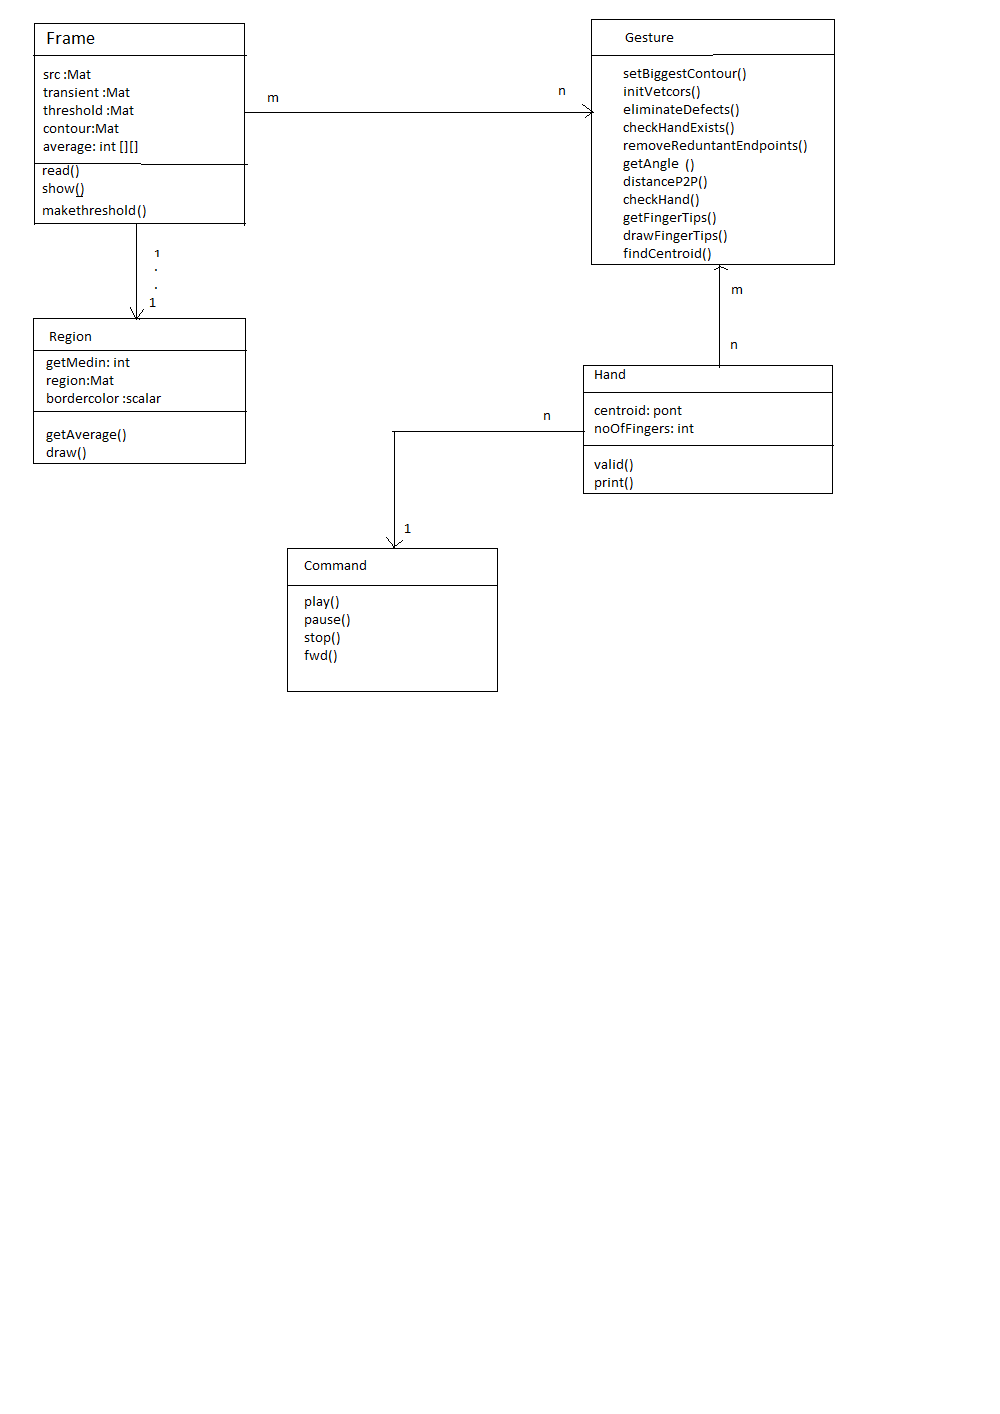
\includegraphics[width=10cm]{images/class.png}\\
						\caption{Class Diagram}
			\end{centering}
		\end{figure}
		\newpage
			\subsubsection{Code Overview}

					We have written the code as .cpp and .hpp files. A lot of files were included in order to increase the modularity. We have done all the definitions and the declarations in the hpp files. 

					\mparagraph{Class frame:\\}

						This class is to do the functions associated with the frame and store them. Frame read and frame display functions are defined in this class. 

						\paragraph{Variables:\\}
						 Mat src: Initially read matrix\\
   						 Mat transient: The matrix where all the changes will occur\\
    					 Mat threshold: The matrix black and white matrix threshold\\
   						 Mat contours: do stuff with contours\\
    					 int average[7][3]:  The average, lower bound and upper bound color found after average function\\
   					     VideoCapture cap:Capture object to get video from\\

   					    \paragraph{Functions:\\}
   					     \textbf{makeThreshold()\\}
   					     	This function is used to find the threshold matrix. That is done with the help of the average colour detected from another function. With a specified value, the average colour is added and subtracted to get a range. All the colours that come within the range is considered as one and all other as zero. We are iterating through the required regions, whose average is found from the functions defined in the region class which will be mentioned later. The values obtained in each iteration is added into a vector, and the values are ORed and the final output is returned, that is the threshold matrix.\\\\
   					     \textbf{read()\\}
   					     	This function is used to read the frames. The frames are read from a videocapture object, cap. Then it is stored in the src matrix.\\\\
   					    \textbf {show()\\}
   					      	This function is used to display the frame. The source frame is shown at first, and the size of the image is enhanced to show other images on the right side. That is the image when converted to HLS, that image is shown at first, and the display updates when the makeThreshold() function is called. For that a boolean value is set up. If the corresponding boolean value is set, then the threshold image is also shown in the right side.
   					\mparagraph{Class region:\\}

						This class is to do the functions associated with the regions from which the average colour is obtained. 

						\paragraph{Variables:\\}
						
        					Mat region:  The region\\
        					int length: length of region\\
        					Scalar borderColor: Color of the region \\
        					int borderThickness: border is drawn in  border thickness when drawing\\
        				\paragraph{Major Functions:\\\\}
        				\textbf{getAverage()\\}
        					To this function, the source matrix is passed. Then iterating through the region after eliminating the border thickness, the three component values are found separately. And these values are added into a vector during each iteration. So three vectors are obtained. On each of these vectors of h, l and s, the getMedian()function is called. Then the median of each component is returned as the average colour\\
        				\textbf{getMedian()\\}
        					When a vector of values are passed, it sorts the values and returns the mid value.
        			\mparagraph{Class gesture:\\}
        				The gesture class contains the functions from which the contours are detected, fingertips are found etc.\\\\
        				\textbf{Major Functions:\\}\\
        				 \textbf{setBiggestContour()\\}
        				 	The in-built function findContour() returns a vector of vector of points. So there are a vector of contours. From that, we assume that the biggest contour is the required one, we find the biggest contour by iterating through every set of contours. Then the biggest contour's index is stored for detecting the contour of interest.\\\\
    					 \textbf{eliminateDefects()\\}
    					 	The defects in the convex hull are found using an openCV's in built function called convexityDefects(). This function returns a vector of defects. From these defects, the unwanted ones are removed using this function. Here an angle tolerance of 95 degree and depth tolerance of height/5 is given. All the defects that are not within this tolerance limits are eliminated.\\
    					 	\\
    					 \textbf{checkHandExists()\\}
    					 	It returns false if the number of fingers are greater than five, if there is no bounding rectangle or if the width to height or height to width ratio is greater than four. It returns true for all other values.\\
    					 	\\
    					 \textbf{removeRedundantEndPoints()}
    					 	This function is called after eliminateDefects(). Here the points within close proximity are removed. Here a value for angle tolerance, and distance tolerance is provided. The values coming outside the tolerance limit is removed from the list of removed defects.\\
    					 	\\
    					 \textbf{getAngle()\\}
    					 	To this function, three points are passed. The angle subtended by the second point when two lines are drawn from second point to first point and second point to third point is found. The it returns the radian value of the given angle. \\
    					 	\\
    					 \textbf{distanceP2P(Point, Point)\\}
    					 	Returns the algebraic distance between the two points by taking the square root of the sum of squares of difference of x coordinates of two points and that of y coordinates.\\
    					 	\\

					     \textbf{getFingerTips()\\}
					     	The convexityDefect() returns a vec4i value. There is a start point, end point and farthest point. So if there is a farthest point in between, the start and points are fingertips. First, if there is no finger, add the first point and for all other iterations add the end points From this function number of fingers are also tracked.\\\\
					     \textbf{drawFingerTips()\\}
					     	The fingertips returned by the previously defined function is drawn with the help of this function. It iterates number of fingers times and takes the points of each finger and draws it.\\\\
    					 \textbf{findCentroid()\\}
    					 	The centroid of the gesture is found using this method.\\\\
    				\mparagraph{Class Hand:\\}
    					In this class, number of fingers and coordinates of each of them are printed and also checks if the hand is valid.
    				\mparagraph{Class Command: \\}
    					In this class, the in built functions of VLC operations in the VLC library are included. \\\\
    					\textbf{Major Functions: \\\\}
    					\textbf{getCommand()\\}
    						This is a class to display all the functions, all the function numbers and also the gesture as a description.\\\\
    					\textbf{doCommand()\\}
    						In this function, we get a value returned from the recogniseCommand() function. Thus this function calls the inbuilt function which is associated with the returned value.\\\\
    					\textbf{recogniseCommand()\\}
    						To this function, a vector of hands are passed. And iterating through each of the hands, the movement of the x coordinate of the centroid is tracked. If the centroid moves to the right, the number corresponding to the play function is returned. If the centroid moves to the left, the number corresponding to the pause function is returned.
    						If the centroid is not changing, the fingertip motion is calculated, using the variation in the x and y coordinates of the fingertips of the successive hands. If the x coordinate is increasing and y coordinate is decreasing, the number corresponding to the forward function is returned . If x is decreasing and y is increasing, the number associated with the stop function is returned.

 	\section{Results and Discussions}
 		When the hand is shown, after the average colour is found out, and filtering is done, the threshold image is found. Although background conditions and lighting conditions created problems, clear threshold images are obtained if the background and the skin colour are almost different to each other. In other conditions also, approximate binary images are available.

 		With this, if the threshold image is correct, the contours are also obtained clearly. Convex hull is drawn to understand the outer region of the hand, and then defects are also found. After this, we obtained the fingertips and its coordinates also.

 		With the help of recognised gesture, we could execute the commands. Certain commands were not obtained clearly if the obtained threshold image is less accurate. But almost static background conditions and less noise, threshold and hence the commands are obtained appropriately. 
			
		\subsection{Screenshots}
		\begin{figure}[!ht]
			\begin{centering}
				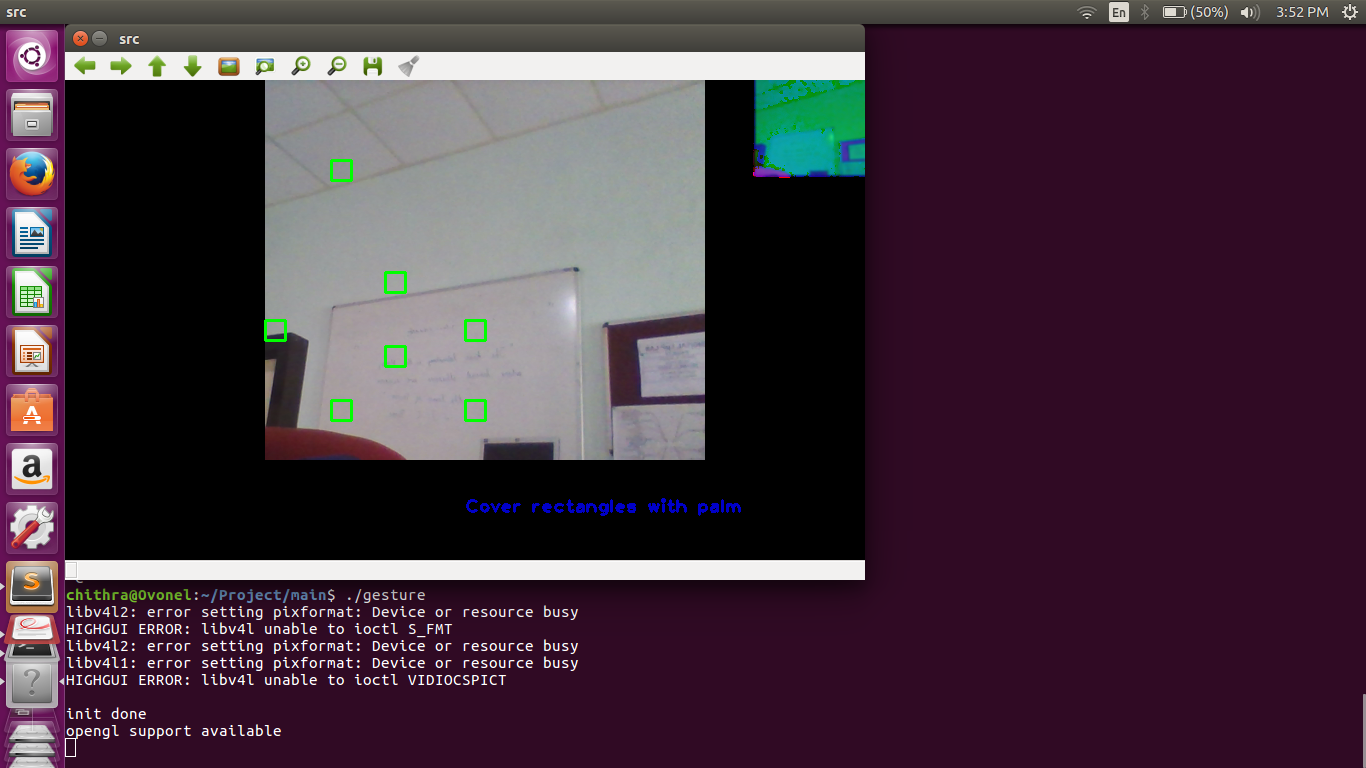
\includegraphics[width=10cm]{images/region.png}\\
						\caption{A set of regions are shown to show our hand}
			\end{centering}
		\end{figure}
		\begin{figure}[!ht]
			\begin{centering}
				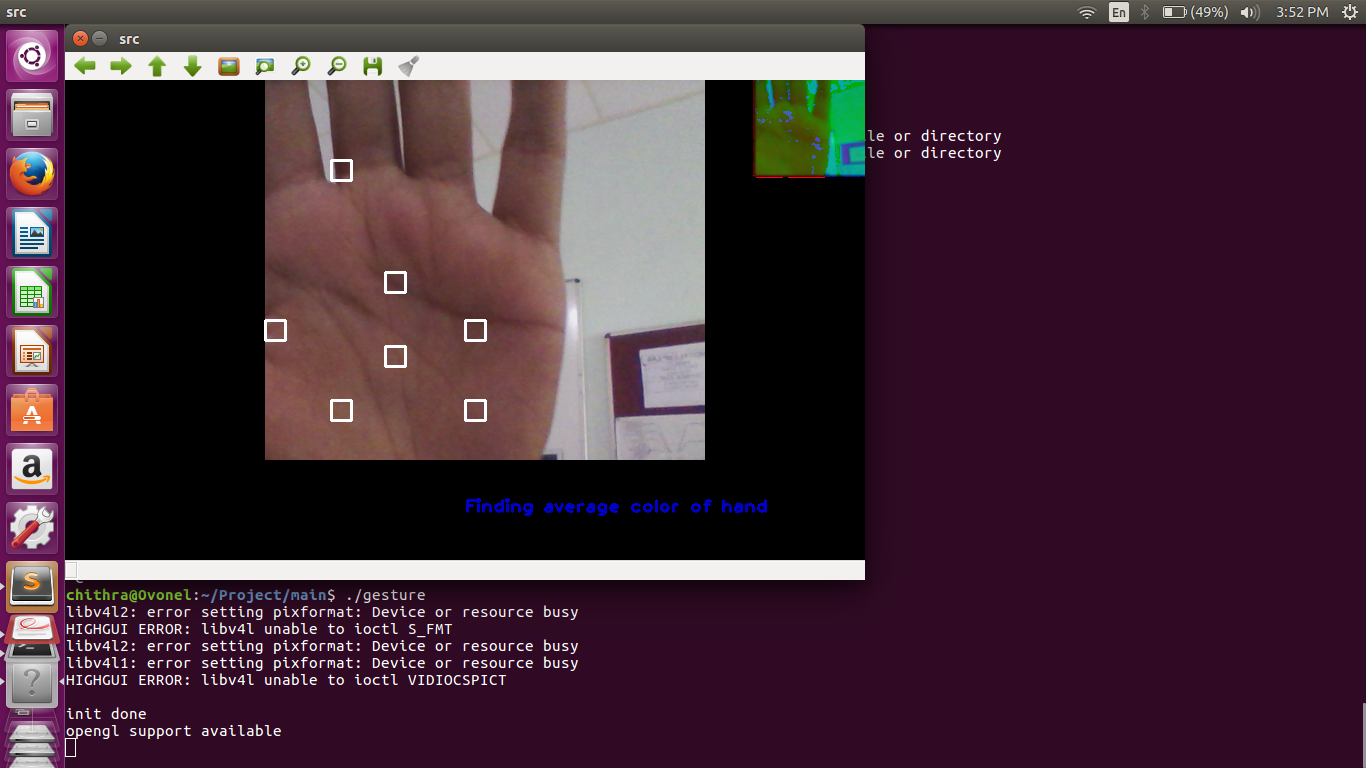
\includegraphics[width=10cm]{images/avg.png}\\
						\caption{Detection of skin colour}
			\end{centering}
		\end{figure}
		\begin{figure}[!ht]
			\begin{centering}
				
\includegraphics[width=10cm]{images/hand.png}\\
						\caption{Detection of fingertips of hand}
						Fingertips, number of fingers and the centroid are shown
			\end{centering}
		\end{figure}
		\newpage

		\begin{figure}[!ht]
			\begin{centering}
				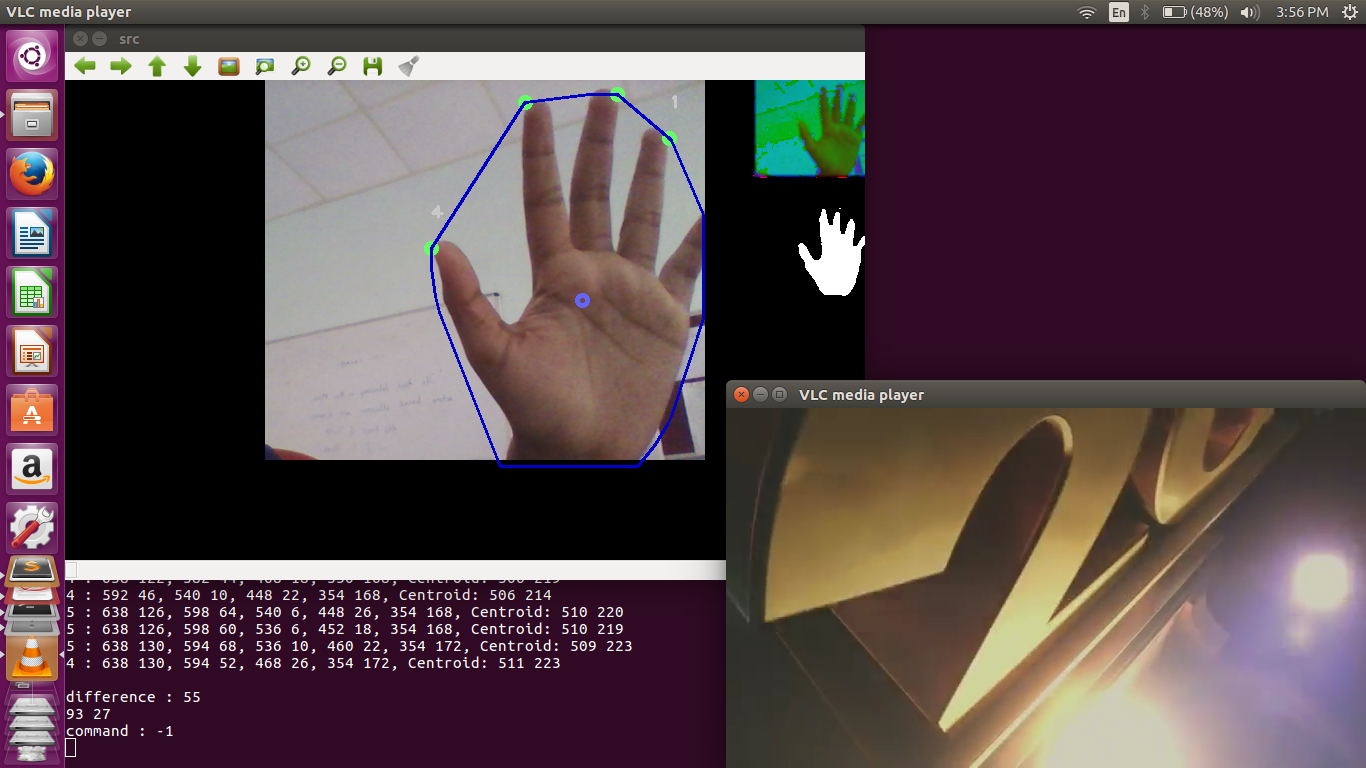
\includegraphics[width=10cm]{images/play.png}\\
						\caption{Swipping hand to right}
						When swiped to right, video plays(the process  currently being executed is printed in terminal)
			\end{centering}
		\end{figure}

		\begin{figure}[!ht]
			\begin{centering}
				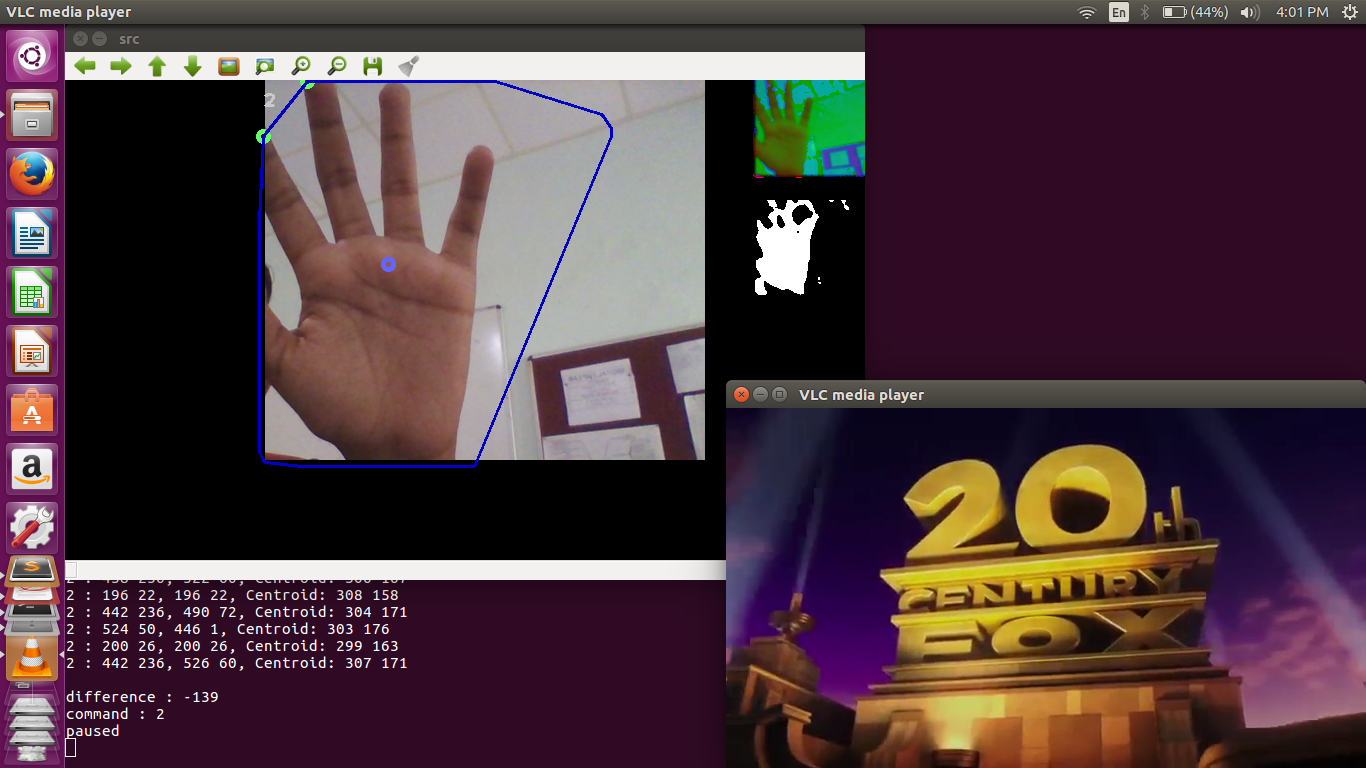
\includegraphics[width=10cm]{images/pause.png}\\
						\caption{Swipping hand to left}
						When swiped to left, video pauses(the process currently being executed is printed in terminal)
			\end{centering}
		\end{figure}
		\newpage
		\begin{figure}[!ht]
			\begin{centering}
				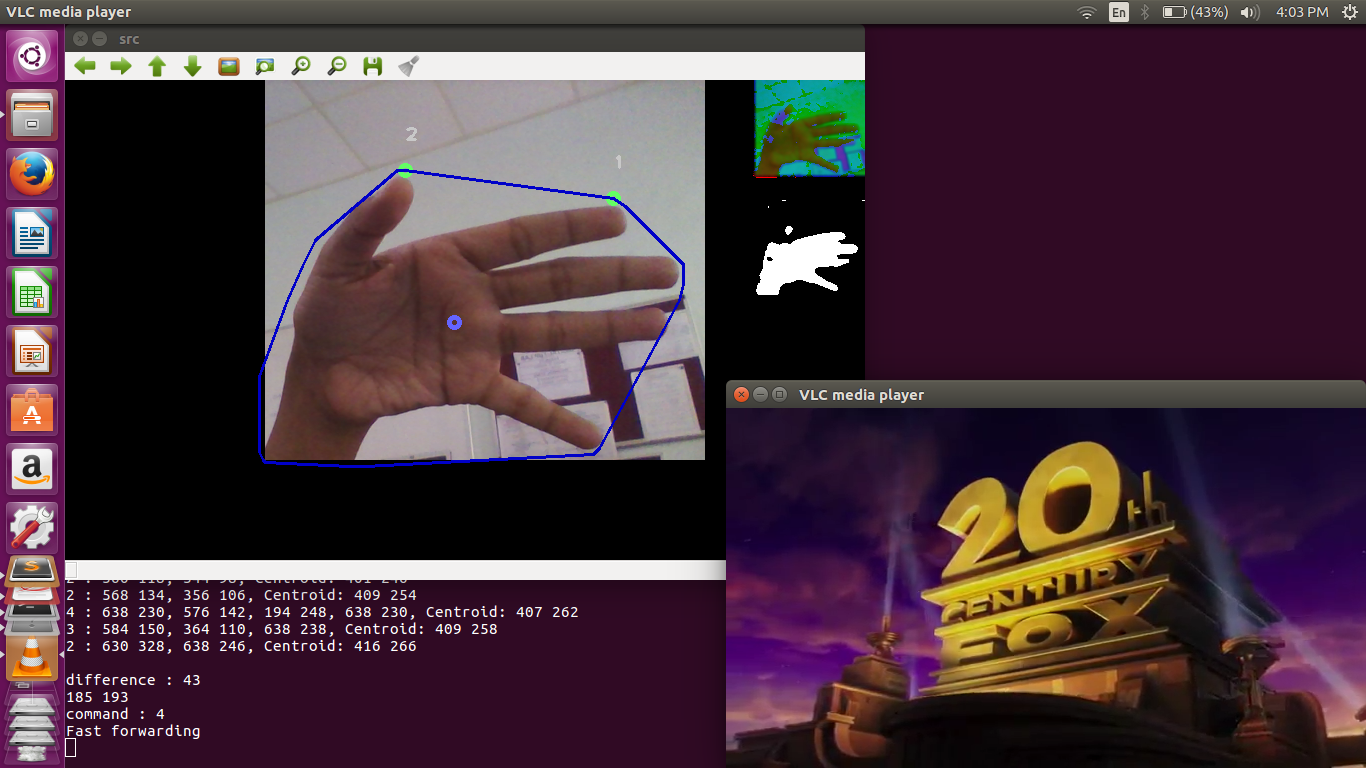
\includegraphics[width=10cm]{images/fwd.png}\\
						\caption{Tilting hand to right}
						When tilted to right, video forwards(the process currently being executed is printed in terminal)
			\end{centering}
		\end{figure}
		
		\begin{figure}[!ht]
			\begin{centering}
				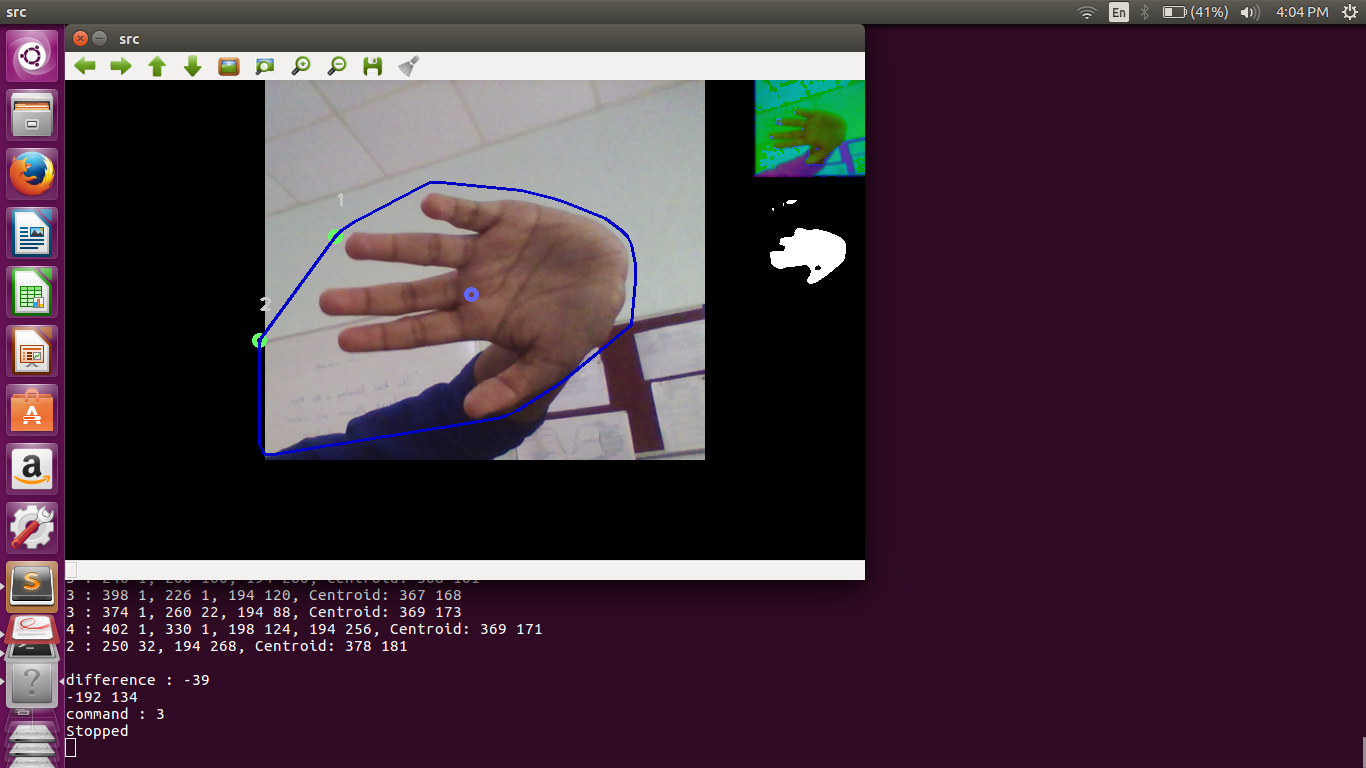
\includegraphics[width=10cm]{images/stop.png}\\
						\caption{Tilting hand to left}
						When tilted to left, video stops(the process currently being executed is printed in terminal)
			\end{centering}
		\end{figure}
		\newpage
		
			
	\section{Further Work}

			Gestures  are  destined  to  play  an  increasingly  important  role  in  human-computer  interaction  in  the future.Area of Hand gesture based computer human interaction is very vast. Hand recognition system can be useful in many fields like robotics, computer human interaction.

			As we have included simple gestures now, as further enhancement, we will try to implement complicated gestures by taking more features of the gesture rather than fingertip movement and centroid. In the enhanced method, we will try to take features like size, distance from different sides of the frame etc. 

			Another enhancement we are trying to implement is that the HGR can be used to control other applications rather than VLC. For easiness, we can set gestures for opening application etc.
			Also, various sign languages can also be interpreted using this technique. As gestures are user friendly, it will be nice to make the Human Computer Interaction more flexible. 
			
	\section{Conclusion}
		It  is  concluded  that  gesture  is  most  basic  and  natural  part of  the  human interaction. So using gesture as communication medium between human and computer will help to bridge the real word with digital world. Moreover to use this system there is no need of extra sensors or hardware, which make this system cost efficient and simple. And anyone can use this system with simple training. Hence it is fair to say that this system will play vital role in advancement of Human Computer Interaction (HCI) and will be a milestone in User Interfacing.
		
		Hand gesture recognition and related fields of image processing and computer vision is gaining relevance in various areas. Through this project, we have tried to enhance the usage of digital world by controlling the VLC media player app. We have shown a prototype model with by tracking the dynamic gestures in different backgrounds. We have taken both the hand movement and fingertip movements. The basic operations of VLC are controlled currently. We have used gestures as a way to ease the users. 

% 		\section{References}


% 		1
% 2.

% 3.
% Qing Chen Nicolas, D. Georganas, Emil M. Petriu, "Hand Gesture Recognition Using Haar-Like Features And A Stochastic Context-Free Grammar" in , IEEE, vol. 57, no. 8, August 2008.

	\newpage
	\nocite{*}
	\bibliography{helpers/bibliography}
	\bibliographystyle{ieeetr}

\end{document}